\clearpage
\section{Method}
\label{sec:method}

Our method is split into to two parts, the routing algorithm and the accessibility analysis tool.
Our routing algorithm is an applied version of MCR with minor variation to make it more suitable in terms of free-floating vehicle sharing.

% requirements on routing algorithm
% - unrestricted
% - multi-modal (must incorporate scheduled networks (public transfer) and an arbitrary number of other unscheduled networks)
% - multi-objective (must be able to incorporate an arbitrary amount of objectives), whose values update based on the previous values and the current edge (either unscheduled network edge or trip between two stops)
% - inter-modal (the different transport modes may be sequenced in any order (not just bicycles for start and end)

In order to fully grasp the potential of the combination of the sustainable modes of transport, we require our routing algorithm to be \textbf{multi-modal}, \textbf{multi-objective}, and \textbf{unrestricted inter-modal}, and run in a reasonable time.

\textbf{Multi-modal} means that our routing algorithms allows multiple modes of transport, including scheduled transport systems, like public transfer and an arbitrary number of unscheduled transport systems, like walking, cycling and driving.
In addition we require that free-floating vehicle sharing systems are incorporated realistically.
That means, that our routing algorithm must consider that switching to a free-floating vehicle is possible at any location, where a free-floating vehicle is available and parking a free-floating vehicle is possible anywhere where it's allowed.
% note: this extra excludes MCR

\textbf{Multi-objective} means that our algorithm must find all pareto optimal journeys according to an arbitrary amount of objectives.
The algorithm must provide the possibility to update the values of any objective whenever a \textit{movement} occurs.
We define a movement either as an edge traversal in an unscheduled network or a step in the route traversal during McRAPTOR.
In the case of an edge traversal the new objective must be a function of the old objective and the edge weights, formally: \(l' = f(l, w(e))\), where \(l\) and \(l'\) are the old and new labels, respectively, and \(w(e)\) are the weights of the edge that is traversed.
In the case of an update during a step of the route traversal, the new objective must be a function of the old objective (to be continued).

\textbf{Inter-modal} means that the different transport modes may be sequenced in any order.
For example, when considering walking, cycling through a bicycle sharing system and public transport, the algorithm needs to consider journeys with bicycle rides between two consecutive public transport trips.
\textbf{Unrestricted} means that the algorithm fully searches the unscheduled network graphs, and does not pose restrictions like a maximum of 10 minutes walking distance.


% handled:
% dijkstra, mlc, raptor, ultra, mcraptor, mcr
% relate to other algorithms
Both Dijkstra and MLC are not considered due to their impractical runtime.
Furthermore, the need for multi-objective solutions excludes Dijkstra, RAPTOR, and ULTRA.
The requirement for unrestricted inter-modal travel makes RAPTOR and McRAPTOR unsuitable in practical scenarios.
To explain this, let's examine a straightforward example.

Consider the OSM graph of the key regions in Cologne, which comprises 125,176 nodes and 142,074 edges.
For RAPTOR to compute a transitively closed graph, it requires calculating the walking distance between each node.
This computation would yield \(125,176^2 = 15,669,030,976\) edges, a number vastly greater than the original 142,074 edges.

While MCR does support multi-objective solutions with unrestricted inter-modal transfers, it doesn't fully encapsulate the multi-modal concept we require.
Although it theoretically permits various modes of unscheduled transport, it is primarily tailored for station-based vehicle sharing systems.
Our focus, however, is on the increasingly prevalent free-floating systems.
In MCR, unscheduled networks are contracted, leading to the removal of certain nodes.
If an optimal route requires a mode change at a deleted node, MCR will be unable to identify that path.
As a result, MCR is not a viable option for our needs.


In the following section, we detail the modifications made to MCR to tailor it to our requirements.

\subsection{Routing Algorithm}
\label{subs:routing_algorithm}

% I/O
The input of our algorithm is a start time and a start node.
The start node may be any node in the OSM network.
The output of our algorithm are the bags for each node in the OSM network.

% Algorithm
% first phase
Our algorithm is split into two phases, which are repeated iteratively.
The algorithm is depicted in Figure \ref{fig:routing_algorithm}.
In the first phase the walking network is explored through the MLC algorithm.
Walking is not considered a trip and there is no upper limit on the walking distance.
In the initial iteration MLC starts with a single label containing the starting values in the bag of the start node.
All other bags are emtpy.
We run MLC until it converges and retrieve the final bags for each node.

% second phase
In the second phase we explore the public transport network, as well as, all modes of unscheduled travel, except walking.
We do so, because a public transport trip, as well as, a trip with any mode of unscheduled travel, except walking will be counted as a trip.

% second phase - RAPTOR
To explore the public transport network, we run one iteration of McRAPTOR.
To retrieve the proper input bags for McRAPTOR we associate each stop in the public transport network with a node in the unscheduled walking network beforehand.
Then we can use the bags of the nodes in the walking network that are associated with a stop in the public transport network as input for McRAPTOR.

% Second phase - MLC
At the same time, we run MLC again, for each unscheduled mode of transport except walking.
For modes based on free-floating vehicle sharing, we use the bags of nodes in the walking network as an input, where a free-floating vehicle is present.
The output is defined depending on where it is possible to drop off vehicles.
If there are no restrictions the bags of all nodes are used.

% merge
The outputs of the McRAPTOR iteration and all MLC runs are merged.
To do so first the output bags have to be translated into the common nodes of the walking network again.
After that the bags are merged according to the merging rules explained in Section \ref{subsubsec:mcraptor}.

The bags that result the merge are the output of the first iteration and contain all optimal labels after exactly one trip.
To obtain the optimal labels after X trips, both phases have to be repeated X times and the result bags of the second phase in iteration \(i\) are used as the input bags of the first phase in iteration \(i-1\).


\begin{figure}
    \centering
    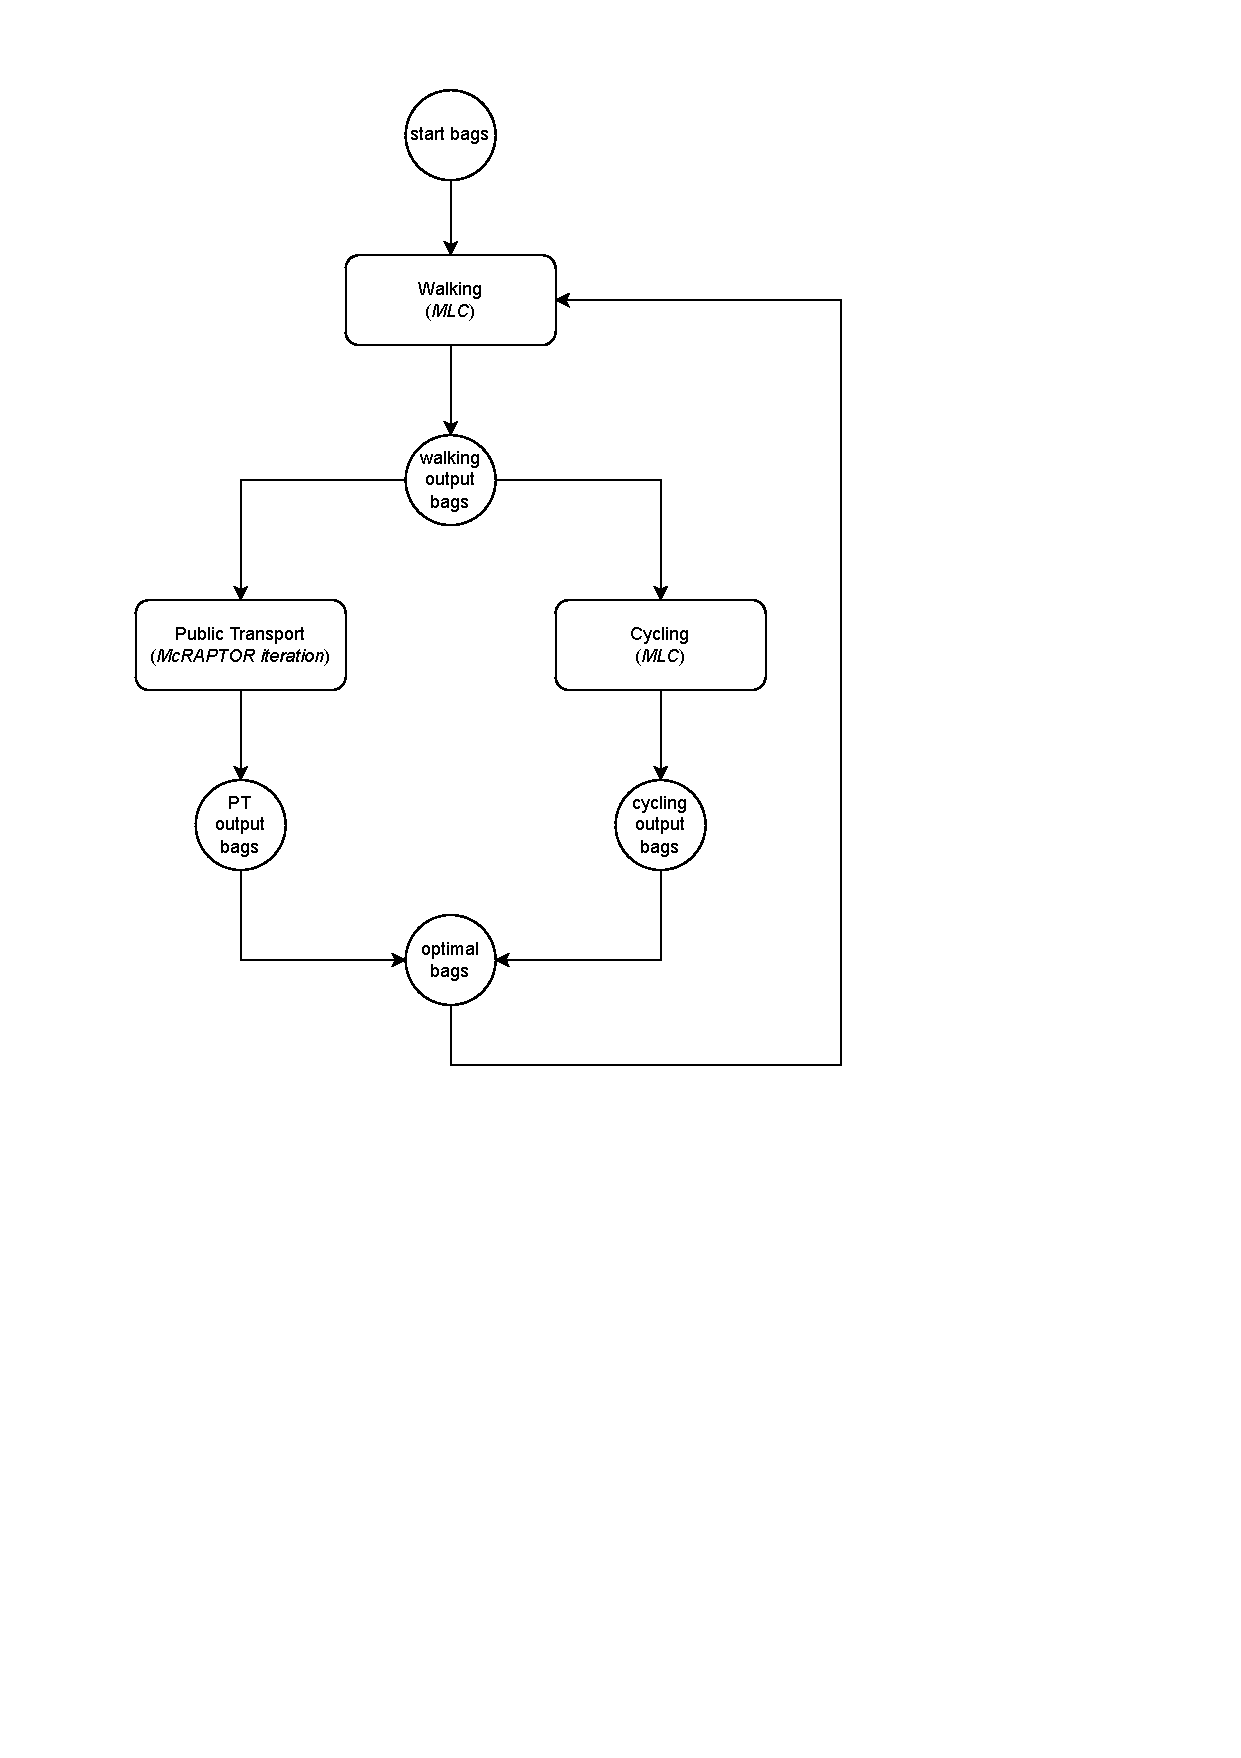
\includegraphics[scale=0.75]{Figures/method/routing_algorithm}
    \caption{Routing Algorithm}
    \label{fig:routing_algorithm}
\end{figure}

\subsection{Data}
\label{subs:data}

\subsubsection{Data Collection}
\label{subs:data_collection}

Our tool requires several datasets as an input: public transport schedules represented by GTFS files, street networks through OSM files, and data that represents free-floating vehicle sharing.
Notably, both GTFS and OSM data can be accessed publicly and can be easily explored, downloaded and preprocessed with the help of our tool.

For GTFS data, we rely on the Mobility Database \shortcite{MobilityDatabase}.
This database serves as an open-source repository containing links to publicly available GTFS feeds globally, standing as the subsequent version of TransitFeeds \shortcite{OpenMobilityDataPublicTransit}.

To use OSM data in practice various tools and services have been developed.
Among these we use, pyrosm \shortcite{Pyrosm} which is a Python library designed specifically for reading OSM data in different formats and conducting data processing operations.
Through pyrosm, we can automatically fetch data from sources like Geofabrik \cite{GeofabrikDownloadServer} and BBBike \cite{BBBikeExtractsOpenStreetMap}, which are two of the most popular OSM data providers.

Using the combination of these resources, our tool ensures easy access to up-to-date GTFS and OSM data.
This allows for easy reproducibility of our results, as well as, the possibility to use our tool for other cities.

\subsubsection{Data Preperation}
\label{subs:data_preperation}

Our tool is able to trim GTFS data to a specific bounding box.
This is especially useful for country-size GTFS feeds.

The GTFS data is also cleaned and converted into a format that is more suitable for RAPTOR.

Specifically, there are two major incompatibilities between the GTFS specification and RAPTOR's notion of routes and trips.
Firstly, each trip belonging to a single route in RAPTOR visits the same stops in the same order.
It is not possible that a trip skips some stops that another trip of the same route visits, much less use a completely different sequence of routes.
In GTFS routes do allow that, as they are much more a group of trips that is presented to the rider under the same name or identifier.
Secondly, GTFS trips allow visiting the same stop multiple times, which is not allowed in RAPTOR.

To overcome these difference our tool splits up routes into smaller routes, that follow the same sequence of stops.
Additionally, it also removes circular trips, altogether.

Similarly, our tool is also able to extract an actual graph from the OSM network.
To do so it utilizes pyrosm.
After extracting the graph from the OSM network, the graph is trimmed to the convex hull of the GTFS stop extended by a small buffer zone.
As a last cleaning step, we remove all nodes, that are not part of the largest weakly connected component.
A weakly connected component is a subgraph in which, if all directed edges were treated as undirected, any two vertices from the subgraph would be connected.
Multiple weakly connected components in graphs derived from OSM data, mostly happen at the border of the considered area and can be neglected.

\subsection{Accessibility Analysis}
\label{subs:accessibility_analysis}

To evaluate the accessibility in cities, we employ a metric that is an implementation of the 15-minute city concept. The concept measures how fast the access to a variety of important amenities is.
To measure this, we categorize amenities into seven essential services: grocery, education, health, banks, parks, sustenance, and shops. (as described by)
Each category is populated with Points of Interest (POIs) sourced from OSM, providing a comprehensive database of locations.

Each service category encapsulates several POIs. For instance, the "Parks" category may include multiple locations tagged in OSM as "leisure: park" or "leisure: dog park".

The core of our metric is the determination of temporal proximity to these amenities. 
For each category, we calculate the minimum travel time required to reach at least one POI of that category. 
The metric is then defined as the maximum value among these minimal times across all categories. 
This approach yields a singular measure that reflects the most significant time distance barrier within an urban area, which effectively captures the least accessible essential service category for any given area.

This metric is critical in assessing the performance of a neighborhood or a city at large against the 15-minute city ideal. It is not an average of accessibility across services but rather highlights the area of greatest need, providing a clear target for urban development and improvement.

By leveraging this metric, we aim to help city planners to create urban environments that prioritize sustainability, enhance the well-being of residents, and reduce dependency on vehicular transport, thus contributing to the broader goals of efficient urban planning and improved quality of urban life.

% explain different modes - this belongs to related work
Traditionally, the 15-minute city concept is applied to walking and or cycling and ignores other modes of transport.
Some researchers, in the context of location-based metrics, even go as far to only calculate the bee-line distance to the nearest amenity and ignore the street network altogether \cite{gastnerOptimalDesignSpatial2006}.

We, however, believe that to accurately determine the accessibility of a city, all modes of transport must be considered, and the routing needs to be as realistic as possible.
We will therefore calculate our metric for various combinations of modes of transport, namely driving with a personal car+walking, free-floating bicycle sharing+walking, public transport+walking, free-floating bicycle sharing+public transport+walking, and walking.
The car mode will serve as a baseline metric and show how competitive more sustainable modes of transport are.

